\documentclass{juliacon}
\usepackage{enumitem}
\usepackage{dsfont}
\usepackage{amsmath}
\usepackage{mathtools}
\usepackage{blkarray, bigstrut}
\usepackage{multirow}

\setlength\parskip{6pt}
\setlist[itemize]{parsep=0pt}
\setlist[enumerate]{parsep=0pt}

\newcommand{\eq}[1]{Equation~(\ref{eq:#1})}
\newcommand{\alg}[1]{Algorithm~\ref{alg:#1}}
\newcommand{\fig}[1]{Figure~\ref{fig:#1}}
\newcommand{\tab}[1]{Table~\ref{tab:#1}}
\newcommand{\lst}[1]{List~\ref{lst:#1}}
\newcommand{\sect}[1]{Section~\ref{sec:#1}}

\setcounter{page}{1}

\begin{document}

% **************GENERATED FILE, DO NOT EDIT**************

\title{Recommendation.jl: A Framework for Building Recommender Systems in Julia}

\author[1]{Takuya Kitazawa}
\affil[1]{Independent Researcher, Canada}

\keywords{Julia, recommender systems, machine learning, evaluation metrics}

\hypersetup{
pdftitle = {Recommendation.jl: A Framework for Building Recommender Systems in Julia},
pdfsubject = {JuliaCon 2022 Proceedings},
pdfauthor = {Takuya Kitazawa},
pdfkeywords = {Julia, recommender systems, machine learning, evaluation metrics},
}



\maketitle

\begin{abstract}
A recommender system is a data-driven application that generates personalized content for users. This paper demonstrates \texttt{Recommendation.jl}, an open-source package for building recommender systems in Julia. In practice, the Julia programming language can be a deeply satisfying option to efficiently and effectively address the recommender's unique characteristics, which rely heavily on repetitive matrix computations in multi-stage data pipelines. To make the systems trustworthy in terms of not only accuracy and scalability but usability and fairness at large, the package provides highly extensible APIs with a diverse set of ready-to-use baseline datasets, recommendation algorithms, and evaluation metrics.
\end{abstract}

\section{Introduction}
\label{sec:introduction}
A recommender system is a type of data-driven, intelligent application addressing the information overload phenomenon on the internet. The application selects top items that are the most likely to be desired by target users under a specific metric, and it assists users' behavior on online services. Most importantly, the foundation of the recommendation engine relies on simple vector and matrix computation against sparse user-item data, where we can take full advantage of numerical computing methods. That is, many classic but still performant recommendation algorithms run on a $|\mathcal{U}|$-by-$|\mathcal{I}|$ user-item matrix $R \in \mathbb{R}^{|\mathcal{U}| \times |\mathcal{I}|}$, where $\mathcal{U}$ and $\mathcal{I}$ are respectively a set of users and items. Notice that $R$ normally shows high sparsity with limited user-item events on massive $|\mathcal{U}|$ and $|\mathcal{I}|$. \fig{recommender} illustrates how user-item data is transformed and processed for making recommendations.

\begin{figure}[htbp]
    \centering
    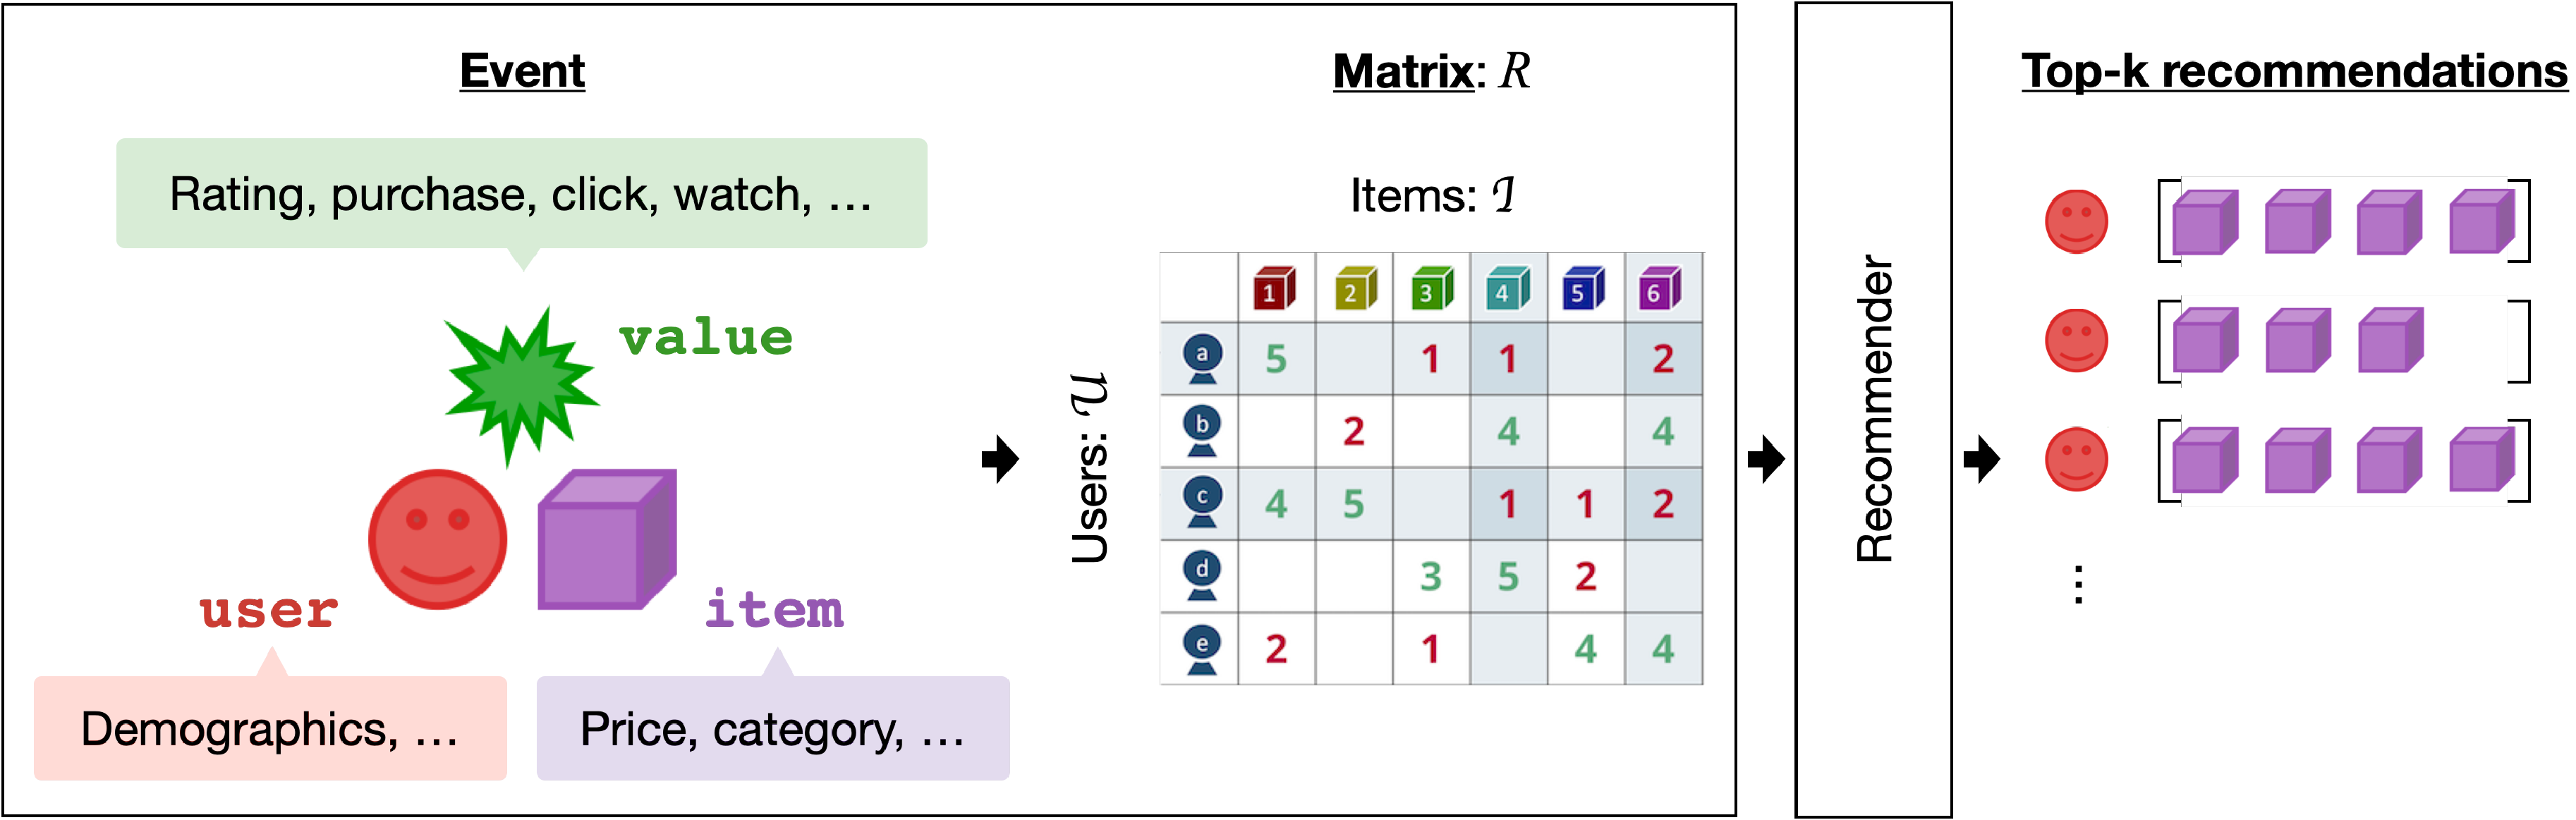
\includegraphics[width=1.0\linewidth]{images/recommender.pdf}
    \caption{Overview of how a recommender works. Event data between users and items are converted into a matrix $R$, which is eventually fed into a recommendation algorithm to generate a ranked list of items per user.}
    \label{fig:recommender}
\end{figure}

Therefore, the Julia programming language that focuses on high-performance scientific computing by utilizing the just-in-time compiler \cite{bezanson2017julia} can be a great choice for developers to efficiently and effectively pre-process user-item data, build a recommendation model, evaluate a ranked list of recommended contents, and post-process the recommendation if needed. Conventionally, MATLAB\footnote{\url{http://www.mathworks.com/}} has been widely used for numerical computing, but it is in some sense inefficient proprietary software. Alternatively, open-sourced Julia's efficient implementation is getting the attention of research communities these days. We can readily use various scientific algorithms in Julia by integrating third-party packages, and its syntax dedicated to vector and matrix computations strongly accelerates algorithm development both in industry and academia. However, when it comes to building recommender systems, there are currently no effective Julia packages that enable us to implement recommendation functionality in an extensible way to the best of the author's knowledge.

For the reasons mentioned above, \texttt{Recommendation.jl}\footnote{\url{https://github.com/takuti/Recommendation.jl/}} has been developed in the unique Julia ecosystem. It should be noted that there are quite a few non-Julia open-source solutions available in the community. To give an example, \texttt{LensKit} \cite{ekstrand2020lenskit} takes full advantage of the NumPy/SciPy-based Python scientific computing ecosystem, which naturally makes rapid development and wider use cases possible. On the other hand, \texttt{MyMediaLite} \cite{gantner2011mymedialite} written in C\# is one of the most classic examples that rely purely on the language's built-in arithmetic operators with file IOs; although the tool maximizes the simplicity and transparency of basic recommendation techniques, it is not straightforward for developers to customize the implementation and apply the advanced techniques for optimizing further. Meanwhile, in Java, \texttt{LibRec} \cite{guo2015librec} implements custom interfaces (e.g., dense/sparse matrices) from scratch, and it allows the tool to ensure high extensibility and support various types of state-of-the-art recommenders. 

Regardless of the choice of package, practitioners will realize the recommender implementation can be broken down into similar sub-components: data, recommender, and metrics. \fig{components} illustrates the point, and the rest of the paper is accordingly organized as follows. First, \sect{data} shows how the package eases data manipulation by providing a unified abstraction layer, namely \texttt{DataAccessor}. Next, \sect{algorithm} reviews a variety of recommendation methods the package supports, including collaborative filtering, matrix factorization, and factorization machines. Moreover, in \sect{evaluation}, we dive deep into some of the recommender-specific evaluation metrics and their implementation in Julia, which enable developers to optimize recommenders against not only standard accuracy metrics (e.g., recall, precision) but non-accuracy measures such as novelty, diversity, and serendipity. Finally, \sect{experiment} provides comprehensive benchmark results for supported recommender-metric pairs to undergo trade-off discussion. 

\begin{figure}[htbp]
    \centering
    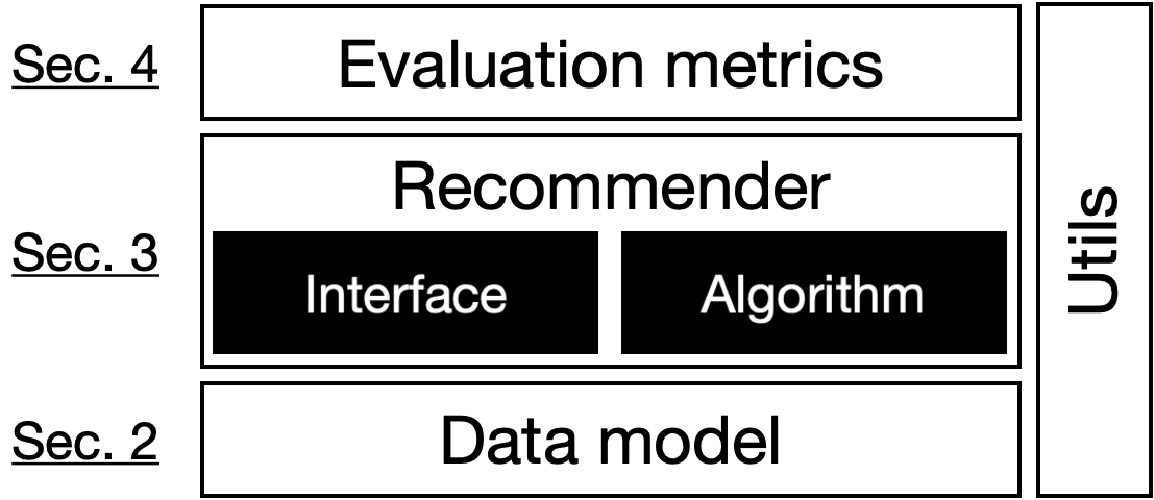
\includegraphics[width=0.5\linewidth]{images/components.pdf}
    \caption{Core components of practical recommender systems. We review each of them throughout the paper.}
    \label{fig:components}
\end{figure}

Ultimately, the contribution of this paper includes but is not limited to (1) demonstrating the Julia-based recommender package that had never existed, (2) sharing the scientific background of the field of recommender systems with the Julia community, and (3) lowering the bar to use the unique programming language in real-world applications as \texttt{Recommendation.jl} has already been used in the hands-on tutorial books \cite{balbaert2019julia,salceanu2018julia}. It should be noted that this paper assumes using \texttt{Recommendation.jl@v1.0.0}, meaning the details might differ in different versions.


\section{Unified Interface for Accessing User-Item Data}
\label{sec:data}
As depicted in \fig{recommender}, a common first step of building a recommender is to capture user-item events and translate them into matrix representation. Here, \texttt{Recommendation.jl} eases the step by providing a unified wrapper called \texttt{DataAccessor}. Since data for recommender systems is easily standardizable as a collection of a user, item, and auxiliary attributes, the common interface helps developers to follow the separation-of-concerns principle and ensure the easiness and reliability of data manipulation. 

To be more precise, raw data is always converted into a \texttt{DataAccessor} instance at the data preprocessing phase with proper validation (e.g., data type check, missing value handling), and hence the subsequent steps can simply take the instance, and access the data (or metadata) without worrying about unexpected input. \fig{accessor} illustrates the procedure.

\begin{figure}[htbp]
    \centering
    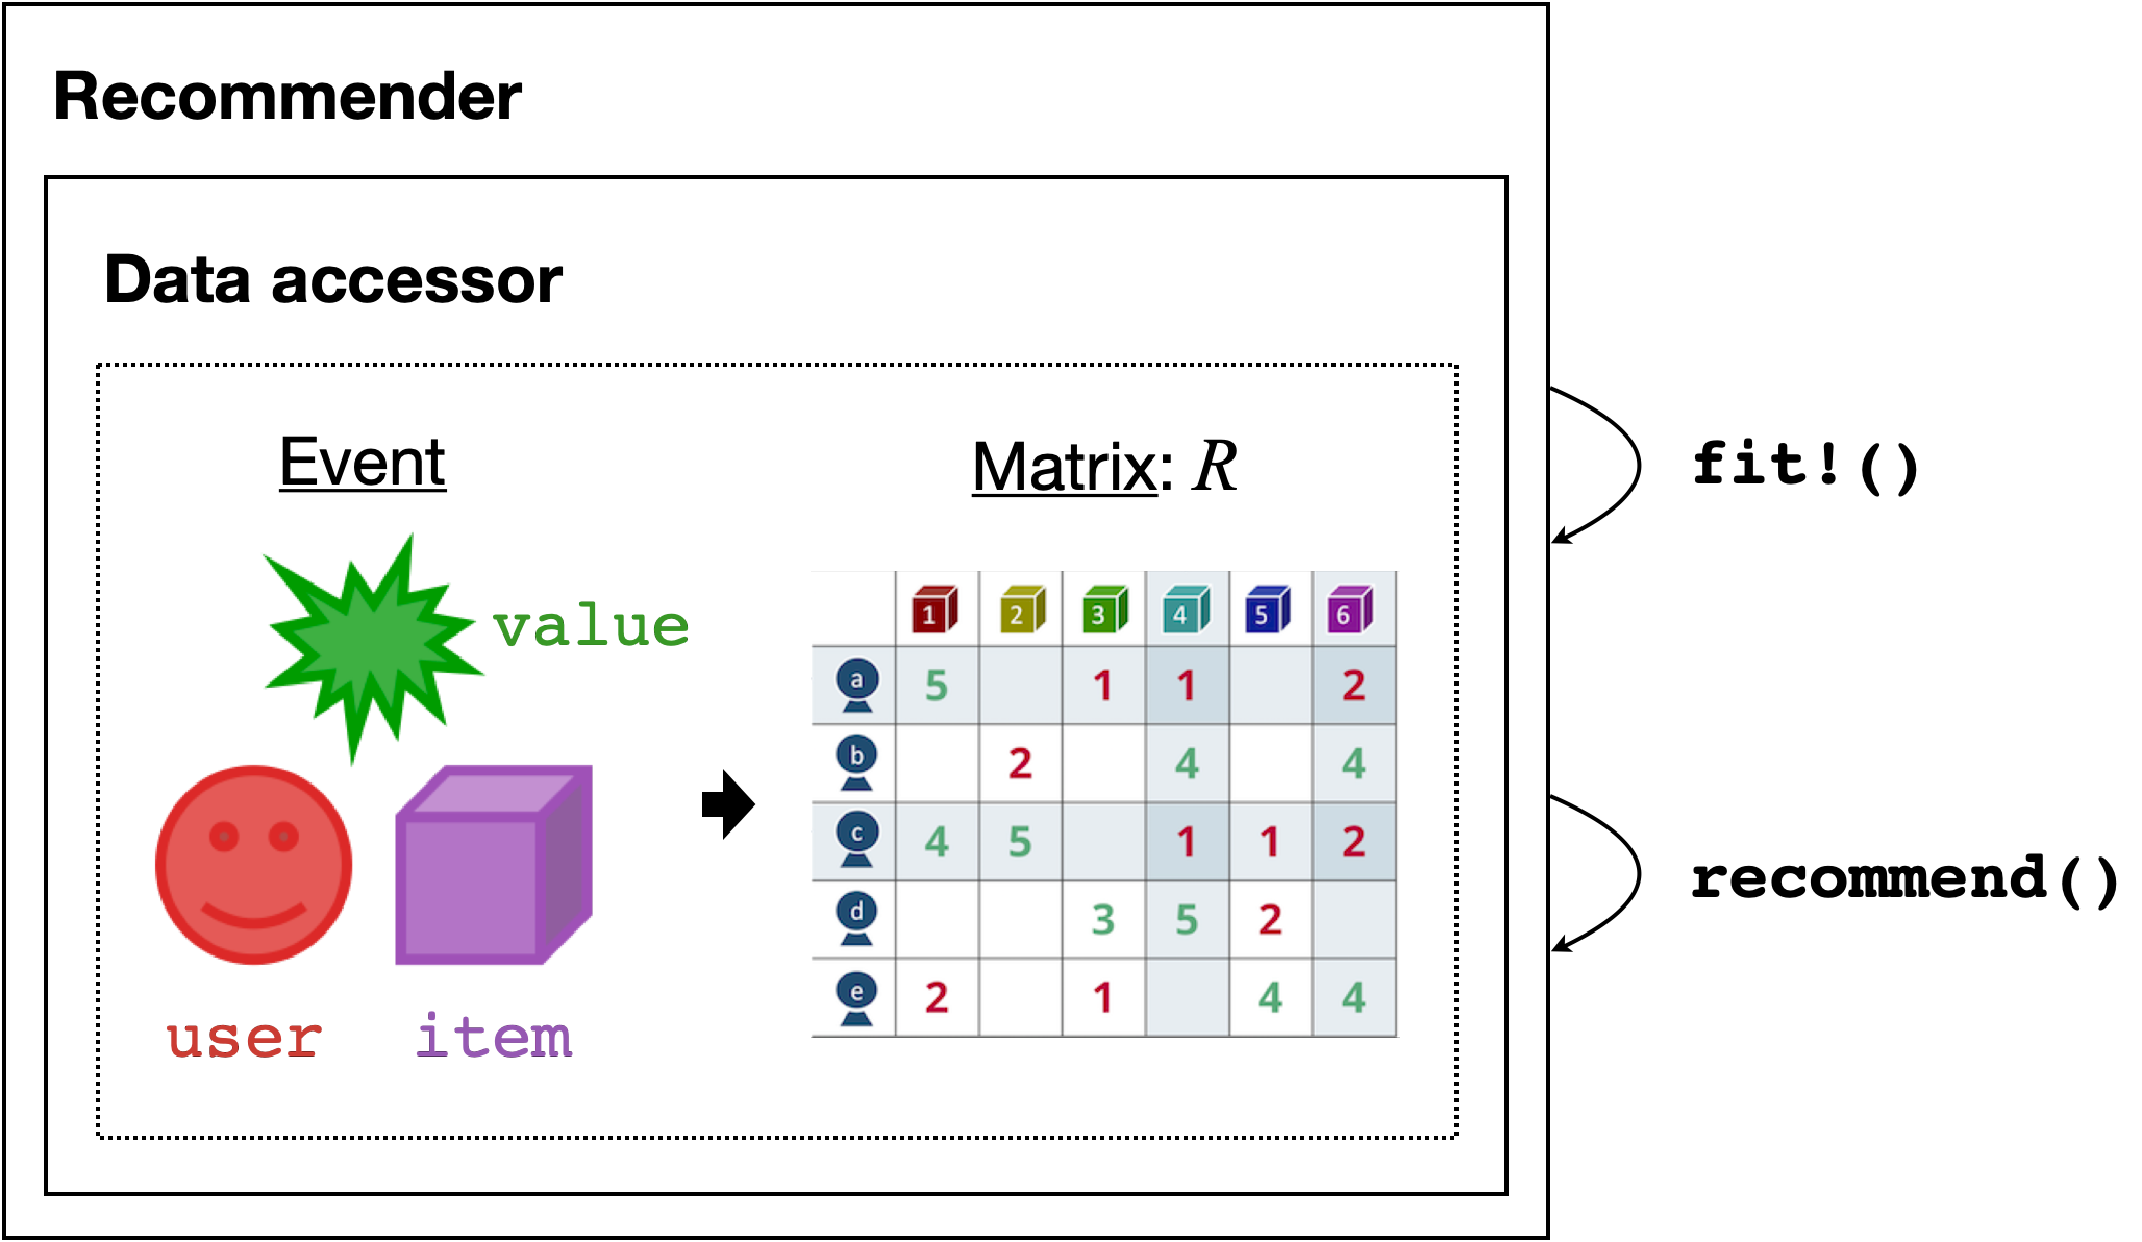
\includegraphics[width=0.8\linewidth]{images/accessor.pdf}
    \caption{\texttt{Recommendation.jl} sees user-item data as a matrix. A recommender runs a training operation \texttt{fit!()} over the data, and a final recommendation list is generated by \texttt{recommend()} based on the trained model.}
    \label{fig:accessor}
\end{figure}

For example, imagine there are 5 users and 6 items on a system, and you observed multiple events:

\begin{lstlisting}[language = Julia]
using Recommendation

n_users, n_items = 5, 6
events = [
    Event(1, 1, 5), # user 1 x item 1
    Event(1, 3, 1), # user 1 x item 3
    # ...
    Event(5, 5, 4), # user 5 x item 5
    Event(5, 6, 4)  # user 5 x item 6
]
\end{lstlisting}

where \texttt{Event} is a composite type for a single user-item interaction:

\begin{lstlisting}[language = Julia]
mutable struct Event
    user::Integer
    item::Integer
    value::Infinite
end
\end{lstlisting}

Note that \texttt{Infinite} is a custom type defined by a union of \texttt{Integer} and \texttt{AbstractFloat}. If \texttt{value} is 0/1 unary integer, such an event is called \textit{implicit feedback,} whereas real numbers like rating value can be seen as the user's \textit{explicit feedback.} Finally, a \texttt{DataAccessor} instance can be created by passing the event list to a constructor as follows, where an array of \texttt{Event} and matrix $R$ are interchangeable.

\begin{lstlisting}[language = Julia]
struct DataAccessor
    events::Array{Event,1}
    R::AbstractMatrix
    user_attributes::Dict{Int,Any}
    item_attributes::Dict{Int,Any}
    
    # constructors
end

data = DataAccessor(events, n_users, n_items)
\end{lstlisting}

In case user (item) data comes with custom attributes such as demographics and contextual metadata, we can use dedicated setter interfaces for enrichment, which allow \texttt{Recommendation.jl} to work with a variety of public and proprietary datasets:

\begin{lstlisting}[language = Julia]
set_user_attribute(data::DataAccessor, 
                   user::Integer, 
                   attribute::AbstractVector)
\end{lstlisting}

Additionally, the package provides data loaders that import publicly available datasets such as MovieLens \cite{harper2015movielens}, Amazon Reviews \cite{ni2019justifying}, and HetRec 2011 Last.FM\footnote{\url{https://www.last.fm/}} dataset \cite{Cantador:RecSys2011}, as well as a synthetic implicit feedback generator using a simple rule-based method demonstrated in \cite{Aharon2013}. These modules return a ready-to-use \texttt{DataAccessor} instance for easing experiments.


\section{Recommendation Algorithms}
\label{sec:algorithm}
As mentioned in \fig{accessor}, a general flow of building recommender systems is (1) taking a list of user-item interactions, (2) applying certain mathematical operations, and (3) finding out top-$k$ most promising list of items for a target user; \texttt{Recommendation.jl} provides standard interfaces \texttt{fit!()} and \texttt{recommend()} to undergo step (2) and (3), respectively. 

\begin{lstlisting}[language = Julia]
abstract type Recommender end

function fit!(recommender::Recommender; kwargs...)
end

function recommend(recommender::Recommender, 
                   user::Integer, topk::Integer, 
                   candidates::AbstractVector{T}
                  ) where {T<:Integer}
end
\end{lstlisting}

That is, among various pre-defined options we see in the following sections, we can choose an arbitrary recommender that inherits the abstract \texttt{Recommender} type. Meanwhile, by implementing a custom concrete subtype like \texttt{MyCustomModel} below and corresponding \texttt{fit!()} and \texttt{recommend()} functions, the developers can build a custom recommendation pipeline on the top of \texttt{Recommendation.jl}. The separation of common interface and actual algorithm implementation makes the package extensible.

\begin{lstlisting}[language = Julia]
struct MyCustomModel <: Recommender 
  data::DataAccessor
end
\end{lstlisting}

In the following sections, we review the basic recommendation algorithms \texttt{Recommendation.jl} natively supports. As previously explained, we delegate data manipulation to \texttt{DataAccessor}, and hence each of the recommendation models simply takes a \texttt{DataAccessor} instance, as well as some recommender-specific optional arguments, through its constructor to be initialized. The fact minimizes the gap between different recommender interfaces and maximizes the usability of \texttt{Recommendation.jl}.

\subsection{Non-Personalized Baselines}

First and foremost, recommender systems are not necessarily built by complex linear algebra or machine learning, and rule-based ``non-personalized'' recommenders are commonly used as a baseline method that derives reasonable recommendations. For instance, regardless of target user's characteristics, a recommender \texttt{MostPopular(data::DataAccessor)} will return top-$k$ most popular items to every user, measured by the number of occurrences (i.e., popularity) in the whole user-item events:

\begin{lstlisting}[language = Julia]
recommender = MostPopular(data)

fit!(recommender)

# for user#4, recommend top-2 from all items
user, topk, candidates = 4, 2, collect(1:n_items)
recommend(recommender, user, topk, candidates)
# -> [item# => popularity] : [4 => 4.0, 6 => 4.0]
\end{lstlisting}

As of writing, the other non-personalized options implemented in the package recommend items: that are most frequently co-occurred with a specific reference item (\texttt{CoOccurrence}), based on a percentage of observed \texttt{Event} values that are greater than a certain threshold (\texttt{ThresholdPercentage}), or based on a global mean of observed \texttt{Event} values (\texttt{UserMean}, \texttt{ItemMean}).

\subsection{Collaborative Filtering}
\label{sec:cf}

Collaborative filtering (CF) is one of the earliest recommendation techniques that was initially introduced in 1992 \cite{Goldberg1992}. The goal of CF algorithm is to suggest new items for a particular user based on a similarity metric. From a users' perspective, CF assumes that users who behaved similarly on a service share common tastes for items. On the other hand, items which resemble each other are likely to be preferred by the same users.

\subsubsection{$k$-Nearest Neighbor}

A $k$-nearest neighbor ($k$-NN) approach, one of the simplest CF algorithms, runs in two-fold. First, missing values in $R$ is predicted based on the past observations. Here, a $(u, i)$ element between a target user $u$ and item $i$ is estimated by computing the similarities of users (items). Second, a recommender chooses top-$N$ items from the results of the prediction step.

Importantly, $k$-NN can be classified into a \textit{user-based} and \textit{item-based} algorithm. In a user-based algorithm, user-user similarities are computed for every pairs of rows in $R$. By contrast, item-based CF stands on column-wise similarities between items. \fig{cf} illustrates how CF works on a user-item matrix $R$. The elements are ratings in a $[1, 5]$ range for each user-item pair, so $1$ and $2$ mean relatively negative feedback and vice versa. In the figure, user $a$ and $c$ seem to have similar tastes because both of them gave nearly identical feedback to item $1$, $4$ and $6$. From an item-item perspective, item $4$ and $6$ are similarly rated by user $a$, $b$ and $c$.

\begin{figure}[htbp]
  \centering
  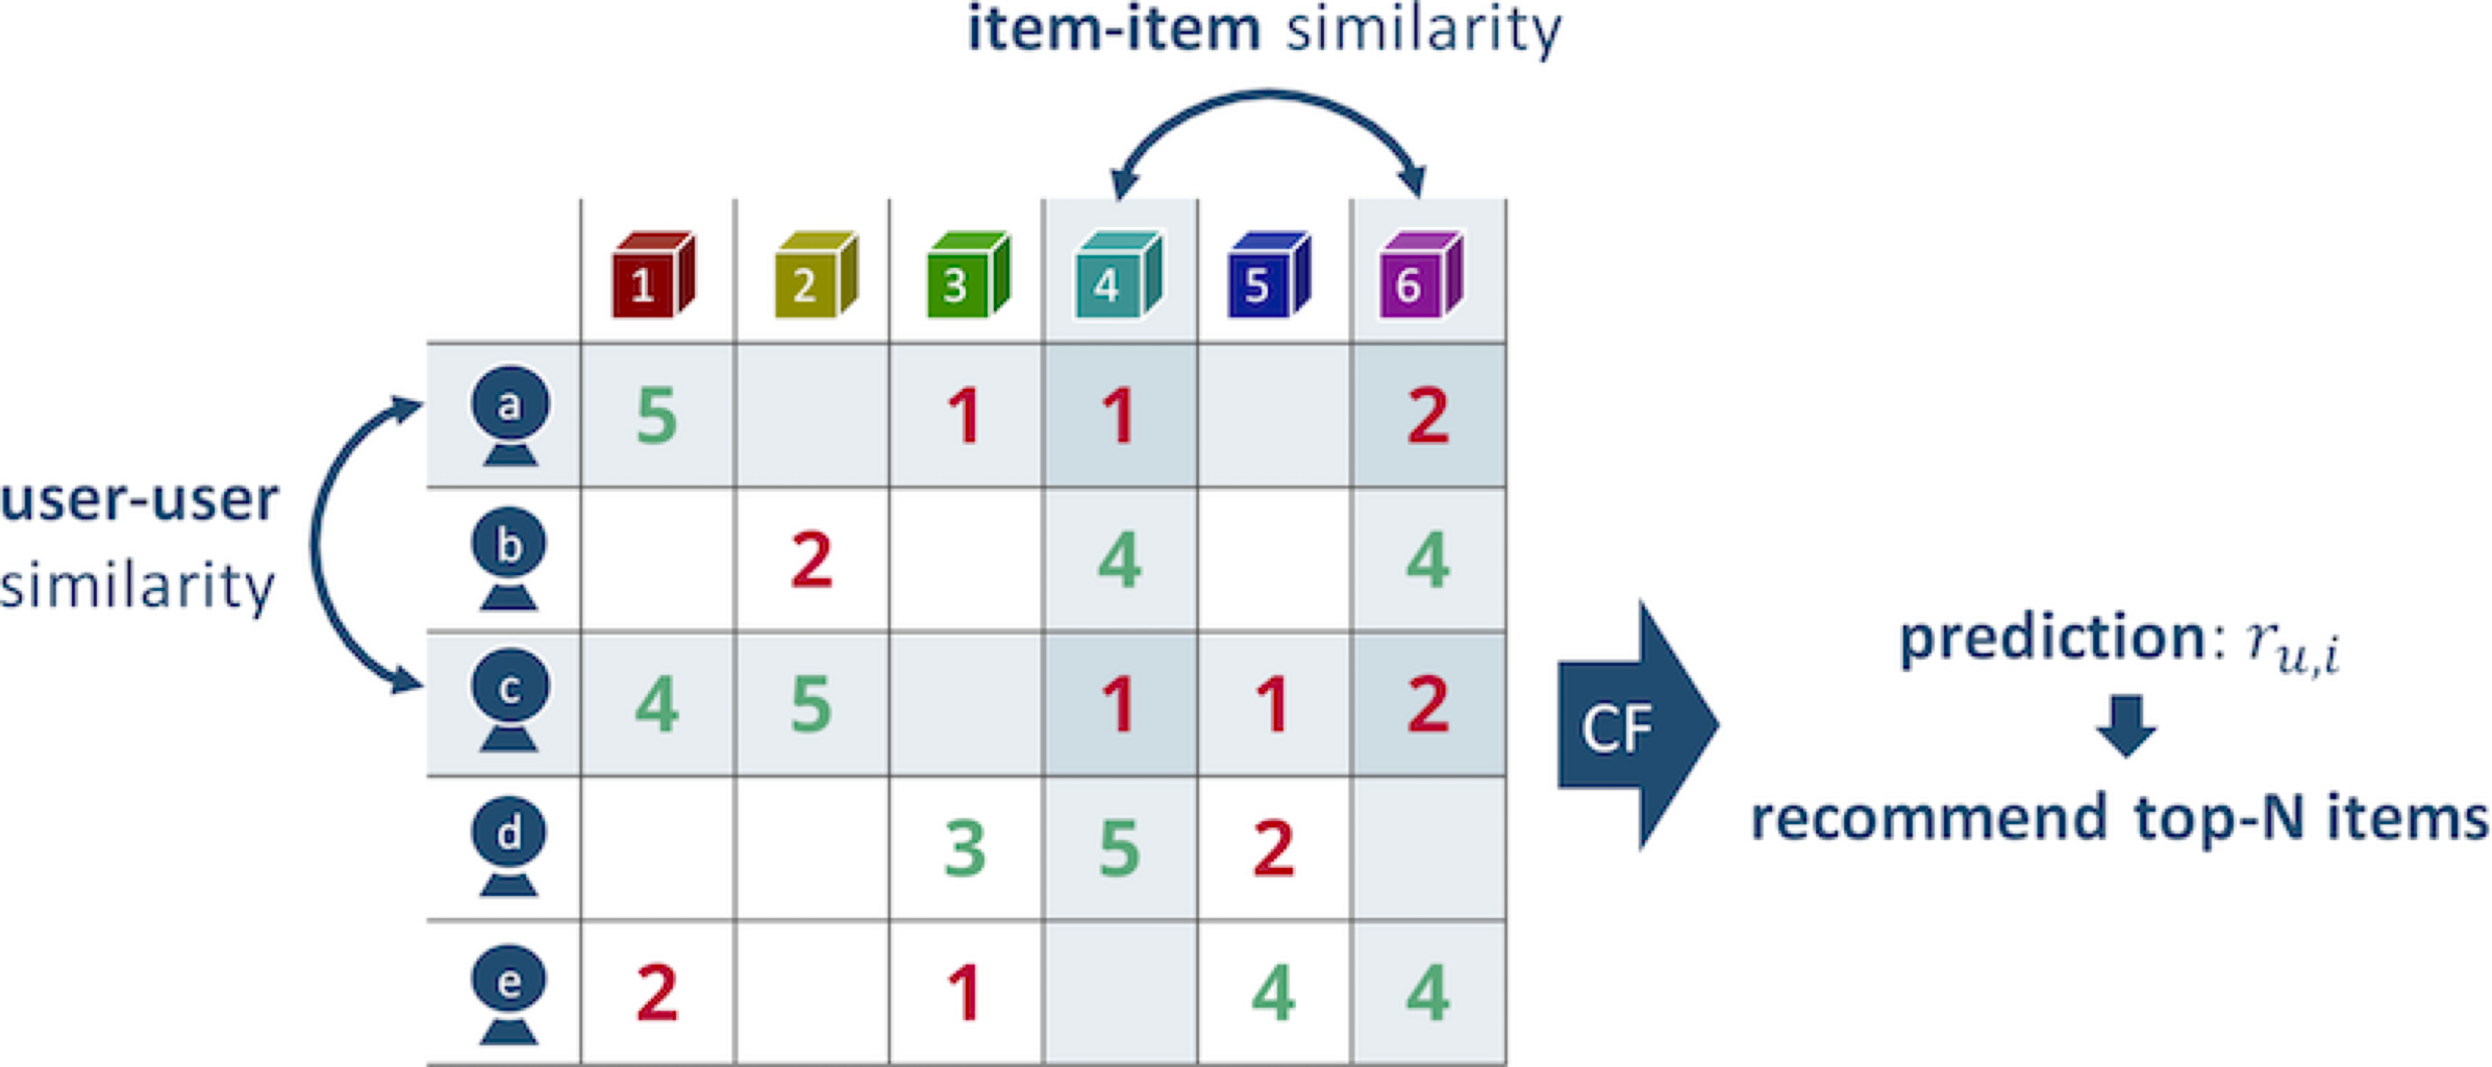
\includegraphics[width=1.0\linewidth]{images/cf.pdf}
  \caption{A schematic diagram of the $k$-NN-based recommender systems on a five-level rating matrix. This figure used Figure~1 in \cite{Sarwar2001} as a reference. For an active user $u$, his/her missing elements $r_{u,i}$ are estimated based on either user-user or item-item similarities, and a recommendation list includes highest-scored items.}
  \label{fig:cf}
\end{figure}

In order to measure the similarities between rows (columns), the Pearson correlation and cosine similarity are widely used. For $d$-dimensional vectors $\mathbf{x}, \mathbf{y} \in \mathbb{R}^d$, the Pearson correlation $\mathrm{corr}(\mathbf{x}, \mathbf{y})$ and cosine similarity $\mathrm{cos}(\mathbf{x}, \mathbf{y})$ are respectively defined as:
$$
\mathrm{corr}(\mathbf{x}, \mathbf{y}) = \frac{\sum_i (x_{i} - \overline{x})(y_{i} - \overline{y})}{\sqrt{\sum_i (x_{i} - \overline{x})^2} \sqrt{\sum_i (y_{i} - \overline{y})^2}},
$$
$$
\mathrm{cos}(\mathbf{x}, \mathbf{y}) = \frac{\mathbf{x} \cdot \mathbf{y}}{\| \mathbf{x} \| \| \mathbf{y} \|} = \frac{\sum_i x_{i} y_{i}}{\sqrt{\sum_i x_{i}^2} \sqrt{\sum_i y_{i}^2}},
$$
where $\overline{x} = \frac{1}{d} \sum^d_{i=1} x_i$ and $\overline{y} = \frac{1}{d} \sum^d_{i=1} y_i$ denote mean values of the elements in a vector. Additionally, in a context of data mining, elements in $\mathbf{x}$ and $\mathbf{y}$ can be distributed on a different scale, so mean-centering of the vectors usually leads better results \cite{Sarwar2001}. Note that cosine similarity between the mean-centered vectors, $\hat{\mathbf{x}} = (x_1 - \overline{x}, x_2 - \overline{x}, \dots, x_n - \overline{x})$ and $\hat{\mathbf{y}} = (y_1 - \overline{y}, y_2 - \overline{y}, \dots, y_n - \overline{y})$, is mathematically equivalent to the Pearson correlation $\mathrm{corr}(\mathbf{x}, \mathbf{y})$, meaning $\mathrm{cos}(\hat{\mathbf{x}}, \hat{\mathbf{y}}) = \mathrm{corr}(\mathbf{x}, \mathbf{y})$, and the following code snippet demonstrates its implementation in the Julia ecosystem.

\begin{lstlisting}[language = Julia]
import Statistics: mean
import LinearAlgebra: dot, norm

function similarity(x::AbstractVector,
                    y::AbstractVector)
    x_hat, y_hat = x .- mean(x), y .- mean(y)
    dot(x_hat, y_hat) / (norm(x_hat) * norm(y_hat))
end
\end{lstlisting}

Based on the similarity definition, user-based CF using the Pearson correlation \cite{Herlocker1999} sees $\mathbf{x}$ and $\mathbf{y}$ as two different rows in $R$, respectively, and gives a weight to a user-user pair by the similarity. In the \texttt{fit!()} phase, the weights allow a recommender to (1) select the top-$k$ highest-weighted users (i.e., nearest neighbors) of a target user $u$, and (2) predict missing elements based on a mean value of neighbors' feedback. Ultimately, sorting items by the predicted values enables \texttt{recommend()} to generate a ranked list of recommended items for a user $u$. Simply put, a constructor of user-based CF in \texttt{Recommendation.jl} is as follows.

\begin{lstlisting}[language = Julia]
UserKNN(data::DataAccessor, n_neighbors::Integer)
\end{lstlisting}

It should be noted that user-based CF tends to be inefficient because gradually increasing massive users and their dynamic tastes require the model to frequently recompute the similarities. On the contrary, item properties are relatively stable compared to the users' tastes, and the number of items is generally smaller than the number of users. Hence, modeling item-item characteristics can be more promising in terms of both scalability and overall accuracy. In particular, the following recommender based on item-based CF \cite{Sarwar2001,Deshpande2004} provides an alternative way of predicting blanks in $R$ based on column-wise item-item similarities in the CF paradigm.

\begin{lstlisting}[language = Julia]
ItemKNN(data::DataAccessor, n_neighbors::Integer)
\end{lstlisting}

\subsubsection{Singular Value Decomposition}

Along with the development of the CF techniques, researchers noticed that handling the original huge user-item matrices is computationally expensive. Moreover, CF-based recommendation leads overfitting to individual taste due to the sparsity of $R$. Thus, dimensionality reduction techniques were applied to recommendation in order to capture more abstract preferences \cite{Sarwar2000}.

Singular value decomposition (SVD) is one of the most popular dimensionality reduction techniques that decomposes an $m$-by-$n$ matrix $A$ to $U \in \mathbb{R}^{m \times m}$, $\Sigma \in \mathbb{R}^{m \times n}$ and $V \in \mathbb{R}^{n \times n}$: 
\begin{align*}
\mathrm{SVD}(A) =& \ U \Sigma V^{\mathrm{T}} \\ 
= & \ \left[\mathbf{u}_1, \mathbf{u}_2, \cdots, \mathbf{u}_m\right] \cdot \mathrm{diag}\left(\sigma_1, \sigma_2, \dots, \sigma_{\min(m, n)}\right) \cdot \\
& \ \left[\mathbf{v}_1, \mathbf{v}_2, \cdots, \mathbf{v}_n\right]^{\mathrm{T}},
\end{align*}
by letting $\sigma_1 \geq \sigma_2 \geq \cdots \geq \sigma_{\min(m, n)} \geq 0$. An orthogonal matrix $U$ ($V$) is called left (right) singular vectors which represents characteristics of columns (rows) in $R$, and a diagonal matrix $\Sigma$ holds singular values on the diagonal elements as weights of each singular vector.

In practice, the most lower singular values of real-world matrices are very close to zero, and hence using only top-$k$ singular values $\Sigma_k \in \mathbb{R}^{k \times k}$ and corresponding singular vectors $U_k \in \mathbb{R}^{m \times k}$, $V_k \in \mathbb{R}^{n \times k}$ is sufficient to make reasonable rank-$k$ approximation of a matrix $A$ as: $\mathrm{SVD}_k(A) = U_k \Sigma_k V_k^{\mathrm{T}}$. It is mathematically proven that $\mathrm{SVD}_k(A)$ is the best rank-$k$ approximation of the matrix $A$ in both the spectral and Frobenius norm, where the spectral norm of a matrix equals to its largest singular value.

\begin{figure}[htbp]
  \centering
  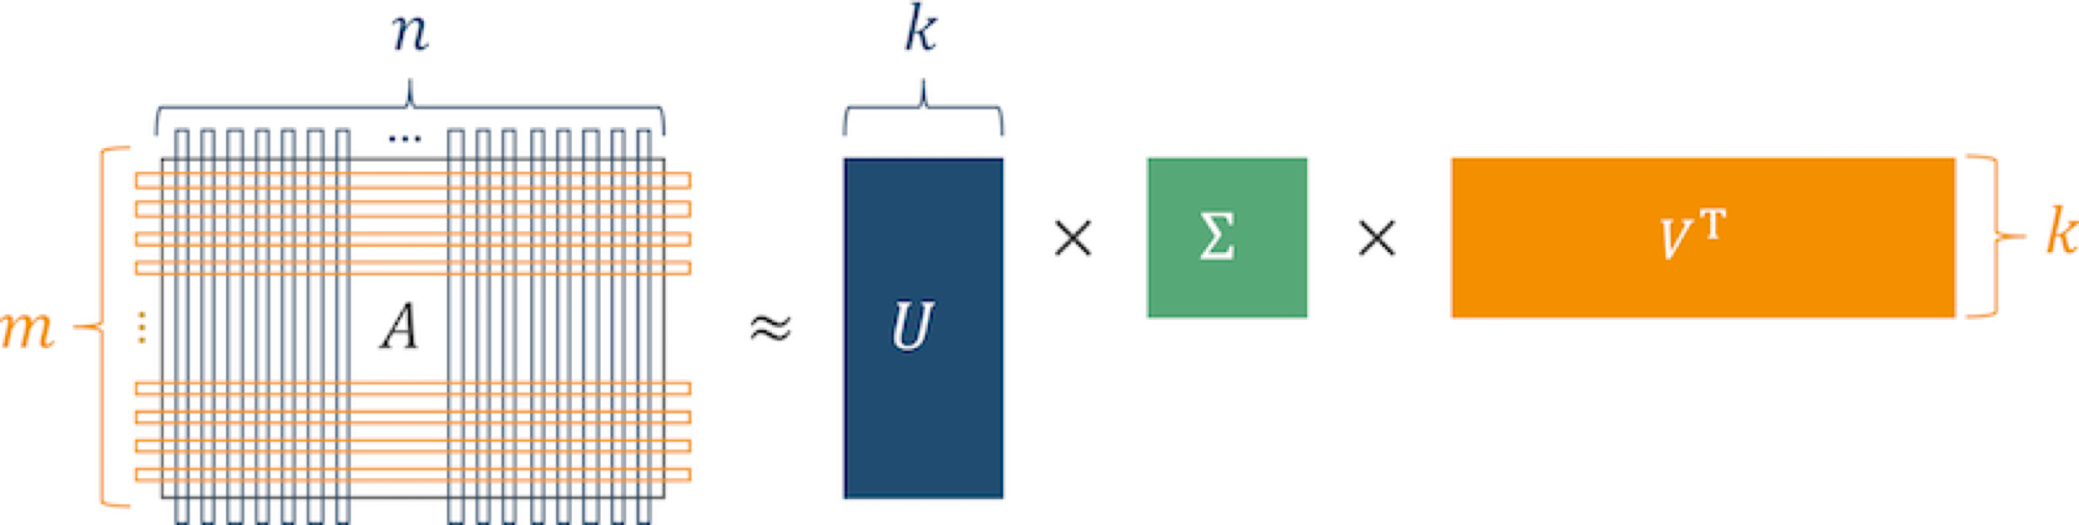
\includegraphics[width=1.0\linewidth]{images/svd.pdf}
  \caption{Rank-$k$ approximation based on SVD. $A \in \mathbb{R}^{m \times n}$ is decomposed into the rank-$k$ orthogonal matrices $U$ and $V$, and diagonal matrix $\Sigma$.}
  \label{fig:svd}
\end{figure}

Sarwar et~al. \cite{Sarwar2000} studied the use of SVD on user-item matrix $R \in \mathbb{R}^{|\mathcal{U}| \times |\mathcal{I}|}$. In a context of recommendation, $U_k \in \mathbb{R}^{|\mathcal{U}| \times k}$, $V \in \mathbb{R}^{|\mathcal{I}| \times k}$ and $\Sigma \in \mathbb{R}^{k \times k}$ are respectively seen as $k$ user/item feature vectors and corresponding weights. The idea of low-rank approximation that discards lower singular values intuitively works as \textit{compression} or \textit{denoising} of the original matrix; that is, each element in a rank-$k$ matrix $A_k$ holds the best \textit{compressed} (or \textit{denoised}) value of the original element in $A$. Thus, $R_k = \mathrm{SVD}_k(R)$, the best rank-$k$ approximation of $R$, captures as much as possible of underlying users' preferences. Once $R$ is decomposed into $U, \Sigma$ and $V$, a $(u, i)$ element of $R_k$ calculated by $\sum^k_{j=1} \sigma_j u_{u, j} v_{i, j}$ could be a prediction for the user-item pair. In the Julia ecosystem, the process can be implemented in a few lines of code with the standard \texttt{LinearAlgebra} library:

\begin{lstlisting}[language = Julia]
import LinearAlgebra: svd
F = svd(data.R)
U, S, Vt = F.U[:, 1:k], F.S[1:k], F.Vt[1:k, :]
# predict a missing value between user and item
r_k = dot(U[user, :] .* S, Vt[:, item])
\end{lstlisting}

\subsubsection{Matrix Factorization}

Even though dimensionality reduction is a promising approach to make effective recommendation, the feasibility of SVD is still questionable due to the computational cost of decomposition and need for uncertain preliminary work such as missing value imputation and searching an optimal $k$. As a result, a new technique generally called matrix factorization (MF) was introduced \cite{Koren2009} as an alternative.

The initial MF technique was invented by Funk \cite{Funk2006} during the Netflix Prize \cite{Bennett07thenetflix}, and the method is also known as \textit{regularized SVD} because it can be seen as an extension of the conventional SVD-based recommendation that gives efficient approximation of the original SVD. The basic idea of MF is to factorize a user-item matrix $R$ to a user factored matrix $P \in \mathbb{R}^{|\mathcal{U}| \times k}$ and item factored matrix $Q \in \mathbb{R}^{|\mathcal{I}| \times k}$, by solving the following minimization problem for a set of observed user-item interactions $\mathcal{S} = \{(u, i) \in \mathcal{U} \times \mathcal{I}\}$:
$$
  \min_{P, Q} \sum_{(u, i) \in \mathcal{S}} \left( r_{u,i} - \mathbf{p}_u^{\mathrm{T}} \mathbf{q}_i \right)^2 + \lambda \ (\|\mathbf{p}_u\|^2 + \|\mathbf{q}_i\|^2),
$$
where $\mathbf{p}_u, \mathbf{q}_i \in \mathbb{R}^k$ are respectively a factorized user and item vector, and $\lambda$ is a regularization parameter to avoid overfitting. Inside of \texttt{fit!()}, an optimal solution can be found by using optimization techniques such as stochastic gradient descent (SGD).

\begin{lstlisting}[language = Julia]
struct MatrixFactorization <: Recommender
    data::DataAccessor
    n_factors::Integer
    P::AbstractMatrix
    Q::AbstractMatrix
end
\end{lstlisting}

Eventually, $R$ is approximated by $PQ^{\mathrm{T}}$ as shown in \fig{mf}, and a recommender can rank items by the  prediction. Notice that mathematically tractable properties of SVD such as orthogonality of factored matrices will be lost over the course of approximation.

\begin{figure}[htbp]
  \centering
  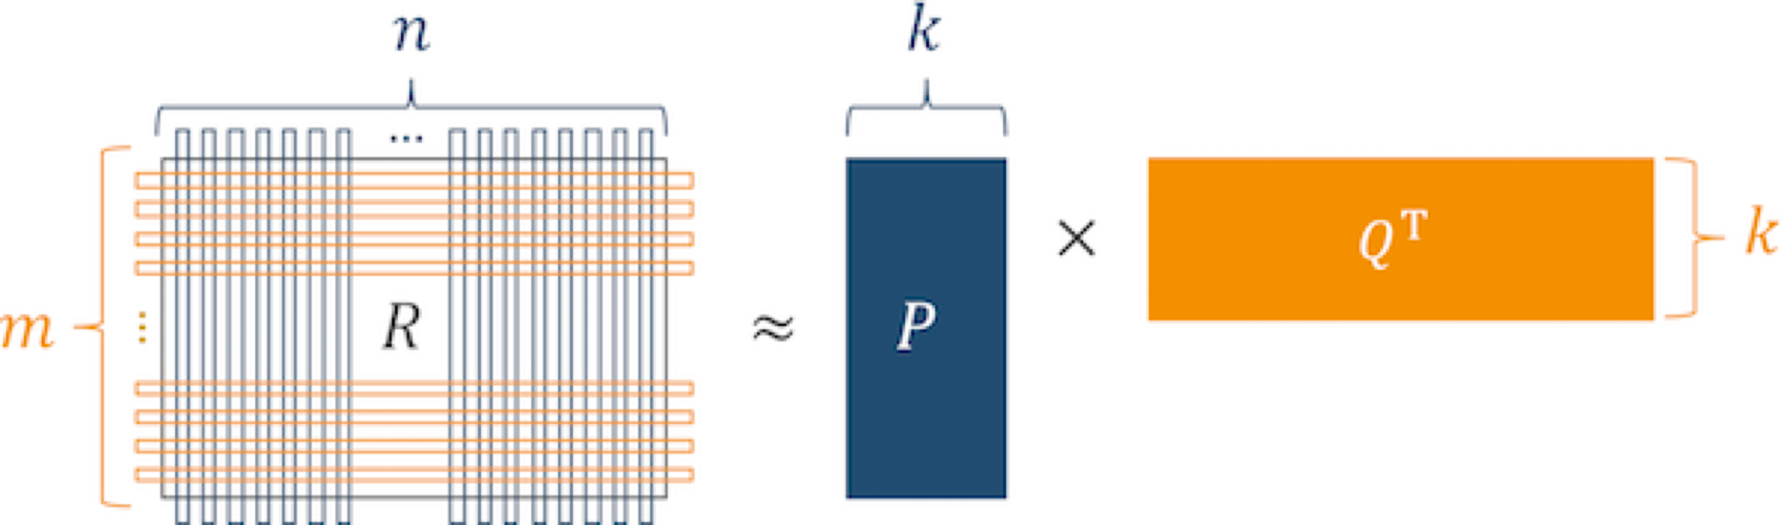
\includegraphics[width=0.8\linewidth]{images/mf.pdf}
  \caption{MF for an $m$-by-$n$ rating matrix $R$. Unlike SVD, singular values in $\Sigma$ are considered to be embedded to the factored matrices.}
  \label{fig:mf}
\end{figure}

MF is attractive in terms of not only efficiency but extensibility. Since prediction for each user-item pair can be written by a simple vector product as $r_{u,i} = \mathbf{p}_u^{\mathrm{T}} \mathbf{q}_i$, incorporating different features (e.g., biases and temporal factors) into the model as linear combinations is straightforward. For example, let $\mu$ be a global mean of all elements in $R$, and $b_u, b_i$ be respectively a user and item bias term. Here, we assume that each observation can be represented as $r_{u,i} = \mu + b_u + b_i + \mathbf{p}_u^{\mathrm{T}} \mathbf{q}_i$. This formulation is known as biased MF \cite{Koren2009}, and it is possible to capture more information than the original MF even on the same set of events $\mathcal{S}$. It should be noted that advanced methods such as tensor factorization \cite{Karatzoglou2010} would require higher dimensionality and more costly optimization scheme to enrich MF.

Meanwhile, there are different options for loss functions to optimize MF. To give an example, Chen et~al. \cite{Chen2011} showed various types of features and loss functions which can be incorporated into a MF scheme. An appropriate choice of their combinations is likely to lead surprisingly better accuracy compared to the classical MF, and \texttt{Recommendation.jl} currently supports Bayesian personalized ranking (BPR) loss \cite{10.5555/1795114.1795167} as an alternative option via \texttt{BPRMatrixFactorization <: Recommender}.

\subsection{Factorization Machines}

Beyond numerous discussions about MF, factorization machines (FMs) have been recently developed as its generalized model. In contrast to MF, FMs are formulated by a equation that is similar to the polynomial regression, and the model can be applied all of regression, classification and ranking problems depending on a choice of loss function with or without SGD-based optimization.

First of all, for an input vector $\mathbf{x} \in \mathbb{R}^d$, let us imagine the following second-order polynomial model parameterized by $w_0 \in \mathbb{R}$, $\mathbf{w} \in \mathbb{R}^d$ as: $\hat{y}(\mathbf{x}) := w_0 + \mathbf{w}^{\mathrm{T}} \mathbf{x} + \sum_{i=1}^d \sum_{j=i}^d w_{i,j} x_i x_j,$ where $w_{i,j}$ is an element in a symmetric matrix $W \in \mathbb{R}^{d \times d}$, and it indicates a weight of $x_i x_j$, an interaction between the $i$-th and $j$-th element in $\mathbf{x}$. Here, FMs assume that $W$ can be approximated by a low-rank matrix $V \in \mathbb{R}^{d \times k}$ for $k < d$, and the weights are replaced with inner products of $k$ dimensional vectors as $w_{i, j} \approx \mathbf{v}_i^{\mathrm{T}} \mathbf{v}_j$ for $\mathbf{v}_1, \cdots, \mathbf{v}_d \in \mathbb{R}^k$. As a result, the formulation of FM model is:
\begin{equation}
\hat{y}^{\mathrm{FM}}(\mathbf{x}) := \underbrace{w_0}_{\textbf{global bias}} + \underbrace{\mathbf{w}^{\mathrm{T}} \mathbf{x}_{ }}_{\textbf{linear}} + \sum_{i=1}^d \sum_{j=i}^d \underbrace{\mathbf{v}_i^{\mathrm{T}} \mathbf{v}_j}_{\textbf{interaction}} x_i x_j.
\label{eq:FMs}
\end{equation}
Several studies \cite{Geuens2015,Rendle2012-1,Rendle2012-3} prove that the flexibility of feature representations $\mathbf{x}$ is one of the most important characteristics that makes FMs versatile. The code snippet below demonstrates how an input vector is created with \texttt{Recommendation.jl}'s utility function \texttt{onehot()}.

\begin{lstlisting}[language = Julia]
x = vcat(
    onehot(1, collect(1:n_users)), # user ID
    onehot(3, collect(1:n_items)), # item ID
    2.5, # rating
    # ...
    onehot("Male", # gender
          ["Male", "Female", "Others", missing]),
    onehot(2, collect(1:7)) # day of week
)
\end{lstlisting}

Note that Rendle \cite{Rendle2012-1} specially referred to \eq{FMs} as \textit{second-order} FMs as a specific case that $p=2$ of the following $p$-th order FMs:
\begin{align*}
\hat{y}^{\mathrm{FM}^{(p)}}(\mathbf{x}) &:= w_0 + \mathbf{w}^{\mathrm{T}} \mathbf{x} \\ &+ \sum^p_{\ell=2} \sum^d_{j_1 = 1} \cdots \sum^d_{j_p = j_{p-1} + 1} \left( \prod^{\ell}_{i=1} x_{j_i} \right) \sum^{k_{\ell}}_{f=1} \prod^{\ell}_{i=1} v_{j_i,f},
\end{align*}
with the model parameters $w_0 \in \mathbb{R}, \ \mathbf{w} \in \mathbb{R}^d, \ V_{\ell} \in \mathbb{R}^{d \times k_{\ell}},$ where $\ell \in \{2, \cdots, p\}$. Although the higher-order FMs are attractive to capture more complex underlying concepts from dynamic data, the computational cost should become more expensive accordingly. In favor of balancing the algorithmic sophistication and its efficiency, \texttt{Recommendation.jl} only considers the second-order model trained by SGD for the time being.

\begin{lstlisting}[language = Julia]
struct FactorizationMachines <: Recommender
    data::DataAccessor
    p::Integer
    n_factors::Integer
    w0::Base.RefValue{Float64} # mutable for fit!()
    w::AbstractVector
    V::AbstractMatrix
end
\end{lstlisting}

\subsection{Content-Based Filtering}

All techniques introduced so far rely on users' historical behavior on a service, but these kinds of recommenders easily face a challenge so-called \textit{cold-start} when it comes to recommending new items (for new users) that do not have sufficient amount of historical data to capture meaningful information. In order to work around the difficulty, content-based recommender systems \cite{Lops2011} are likely to be preferred in reality.

Most importantly, content-based recommenders make recommendation without using the other users' feedbacks. In particular, a content-based approach gives scores to items based on two kinds of information: item model and (static) user preference. In order to model the items, an item-attribute matrix is defined as: $I \in \mathbb{R}^{|\mathcal{I}| \times |\mathcal{A}|}$, where $\mathcal{A}$ is a set of item attributes. Meanwhile, user attributes can be captured through \texttt{DataAccessor}'s \texttt{user\_attributes} property, which is independent from what kind of \texttt{Event}s a system has observed.

From a practical perspective, choosing a set of attributes $\mathcal{A}$ is an essential problem to launch a content-based recommender successfully. In fact, there tend to be numerous candidates on a real-world dataset such as item category and brand, but using too much attributes may increase sparsity and complexity of the vectors, which ends up with poor recommendation performance. With that in mind, one of the most well-studied types of attribute \texttt{Recommendation.jl} also supports is ``term''. More concretely, each item is represented by a set of words, and the items are modeled by TF-IDF weighting \cite{Manning2008}. For instance, if we like to recommend web pages to users, we first need to parse sentences on a page and then construct a vector based on the frequency of each term as:

\begin{equation*}
  I=
  \begin{blockarray}{*{5}{c} l}
    \begin{block}{*{5}{>{$\footnotesize}c<{$}} l}
      apple & banana & candy & $\cdots$ & zoo & \\
    \end{block}
    \begin{block}{[*{5}{c}]>{$\footnotesize}l<{$}}
      3 & 2 & 0 & \cdots & 5 \bigstrut[t]& page\#1 \\
      1 & 0 & 0 & \cdots & 1 & page\#2 \\
      \vdots & \vdots & \vdots & \ddots & \vdots & \vdots \\
      2 & 1 & 8 & \cdots & 0 & page\#N \\
    \end{block}
  \end{blockarray}
\end{equation*}

In case of our item-word matrices, for a given item $i$, term frequency (TF) for a term $t$ is defined as: $\mathrm{tf}(t, i) = \frac{n_{t,i}}{N_i},$ where $n_{t,i}$ denotes an $(i, t)$ element in $I$, and $N_i$ is the total number of words that an item $i$ contains. Meanwhile, inverse document frequency (IDF) is computed over $M$ items as: $\mathrm{idf}(t) = \log \frac{M}{\mathrm{df}(t)} + 1,$ where $\mathrm{df}(t)$ counts the number of items which associate with a term $t$. Finally, each item-term pair is weighted by: $\mathrm{tf}(t, i) \cdot \mathrm{idf}(t)$ in the TF-IDF scheme. 

Since there are several variations of how to calculate $\mathrm{tf}(t, i)$ and $\mathrm{idf}(t)$, \texttt{Recommendation.jl} requires users to pre-compute these numbers in order to maximize the feasibility of the recommender:

\begin{lstlisting}[language = Julia]
struct TFIDF <: Recommender
    data::DataAccessor
    tf::AbstractMatrix
    idf::AbstractMatrix
end
\end{lstlisting}

% If the features were chosen appropriately, content-based recommenders could work well even on challenging settings which cannot be handled by the conventional recommenders. To give an example, when a new item is added to a system, making reasonable prediction for the item is impossible by using the classical approaches such as CF. By contrast, since content-based recommenders only require the attributes of items, new items can show up in a recommendation list with equal chance to the old items. Furthermore, explaining the results of content-based recommendation is possible because the attributes are manually selected by humans.


\section{Evaluation Framework}
\label{sec:evaluation}
One of the notable characteristics of \texttt{Recommendation.jl} is a diverse set of evaluation metrics, including not only the standard accuracy metrics but fairness metrics such as diversity and serendipity. Even though the idea of diverse or serendipitous recommendations is not new in the literature, the topic has rapidly gained traction these days as society realizes the importance of ethical implications in intelligent systems \cite{milano2020recommender}. This section highlights the high-level concept of these metrics and their implementation in Julia based on a common abstract type, \texttt{Matric}.

\begin{lstlisting}[language = Julia]
abstract type Metric end
\end{lstlisting}  

For accuracy metrics, users can use the standard evaluation scheme, \texttt{cross\_validation} and \texttt{leave\_one\_out}, provided by the package. For instance, the following module runs \texttt{n\_folds} cross-validation for a specific combination of recommender and ranking metric. Notice that a recommender is initialized with \texttt{recommender\_args} for making a top-k recommendation.

\begin{lstlisting}[language = Julia]
cross_validation(
    n_folds::Integer, 
    metric::Metric, 
    topk::Integer, 
    recommender_type::Type{<:Recommender}, 
    data::DataAccessor, 
    recommender_args...; 
    # control whether recommending the same item to 
    # the same user multiple times is allowed
    allow_repeat=false
)
\end{lstlisting}

It should be noted that evaluating recommender systems is not always the same as measuring the accuracy of machine learning-based prediction, and there is a separate research domain discussing what an appropriate evaluation method is. In the open-source community, the Python-based \texttt{RecPack} package \cite{michiels2022recpack} considers this point and provides a dedicated layer called \texttt{Scenario}, which can be a future direction \texttt{Recommendation.jl} possibly aims for.

\subsection{Rating Metrics}
\label{sec:rating-metrics}

First and foremost, even though the community focuses more on implicit feedback-based ranking problems lately, rating prediction is still an important foundation in the field of recommender systems as the previous sections mentioned.

\begin{lstlisting}[language = Julia]
abstract type AccuracyMetric <: Metric end
function measure(metric::AccuracyMetric, 
                 truth::AbstractVector, 
                 pred::AbstractVector)
end  
\end{lstlisting}

As a subtype of \texttt{AccuracyMetric}, \texttt{Recommendation.jl} is capable to compute Root Mean Squared Error (RMSE) and Mean Absolute Error (MAE) given pairs of \texttt{truth} and \texttt{prediction} values.

\subsection{Ranking Metrics}
\label{sec:ranking-metrics}

An output from a recommender system is commonly a ranked list of items, and hence measuring the goodness of the ranking is another way to evaluate the systems. 

\begin{lstlisting}[language = Julia]
abstract type RankingMetric <: Metric end
function measure(metric::RankingMetric, 
                 truth::AbstractVector{T}, 
                 pred::AbstractVector{T}, 
                 topk::Union{Integer, Nothing}
                ) where T
end
\end{lstlisting}

Although the interface is the same across the metrics, each of them has a different objective as part of its formulation. To review the differences with some intuition, let a target user $u \in \mathcal{U}$, set of all items $\mathcal{I}$, ordered set of top-$k$ recommended items $I_k(u) \subset \mathcal{I}$, and set of truth items $\mathcal{I}^+_u$. 

\subsubsection{Recall-at-$k$}

Recall-at-$k$ (Recall@$k$) indicates coverage of truth samples as a result of top-$k$ recommendation. The value is computed by the following equation:
$$
\mathrm{Recall@}k = \frac{|\mathcal{I}^+_u \cap I_k(u)|}{|\mathcal{I}^+_u|}.
$$

Here, $|\mathcal{I}^+_u \cap I_k(u)|$ is the number of \textit{true positives} which can be simply computed by the following piece of code:

\begin{lstlisting}[language = Julia]
function count_intersect(
    truth::Union{AbstractSet, AbstractVector}, 
    prediction::Union{AbstractSet, AbstractVector})
    length(intersect(truth, prediction))
end
\end{lstlisting}

\subsubsection{Precision-at-$k$}

Unlike Recall@$N$, Precision-at-$k$ (Precision@$k$) evaluates the correctness of a top-$k$ recommendation list $I_k(u)$ according to the portion of true positives in the list as:
$$
\mathrm{Precision@}k = \frac{|\mathcal{I}^+_u \cap \mathcal{I}_k(u)|}{|\mathcal{I}_k(u)|}.
$$
In other words, Precision@$k$ measures how much the recommendation list covers true pairs.

\subsubsection{Mean Average Precision (MAP)}

While the original Precision@$k$ provides a score for a fixed-length recommendation list $I_k(u)$, mean average precision (MAP) computes an average of the scores against all possible recommendation sizes from 1 to $|\mathcal{I}|$. MAP is formulated with an indicator function for $i_n$, the $n$-th item of $I(u)$, as:
\begin{equation*}
\mathrm{MAP} = \frac{1}{|\mathcal{I}^+_u|} \sum_{n = 1}^{|\mathcal{I}|} \mathrm{Precision@}n \cdot \mathds{1}_{\mathcal{I}^+_u}(i_n).
\end{equation*}
It should be noticed that MAP is not a simple mean of the sum of Precision@$1$, Precision@$2$, $\dots$, Precision@$|\mathcal{I}|$, and higher-ranked true positives lead better MAP.

\subsubsection{Area under the ROC Curve (AUC)}

ROC curve and area under the ROC curve (AUC) are generally used in the evaluation of classification problems, but these concepts can also be interpreted in the context of the ranking problem. The AUC metric for ranking considers all possible pairs of truth and other items which are respectively denoted by $i^+ \in \mathcal{I}^+_u$ and $i^- \in \mathcal{I}^-_u$, and it expects that the ``best'' recommender completely ranks $i^+$ higher than $i^-$.

AUC calculation keeps tracking the number of true positives at different ranks in $\mathcal{I}$. In the implementation of \texttt{measure()}, the code adds the number of true positives which were ranked higher than the current non-truth sample to the accumulated count of correct pairs. Ultimately, an AUC score is computed as a portion of the correct ordered $(i^+, i^-)$ pairs in all possible combinations determined by $|\mathcal{I}^+_u| \times |\mathcal{I}^-_u|$ in set notation. 

\subsubsection{Reciprocal Rank (RR)}

If we are only interested in the first true positive, reciprocal rank (RR) could be a reasonable choice to quantitatively assess the recommendation lists. For $n_{\mathrm{tp}} \in \left[ 1, |\mathcal{I}| \right]$, a position of the first true positive in $I(u)$, RR simply returns its inverse:
\begin{equation*}
  \mathrm{RR} = \frac{1}{n_{\mathrm{tp}}}.
\end{equation*}
RR can be zero if and only if $\mathcal{I}^+_u$ is empty.

\subsubsection{Mean Percentile Rank (MPR)}
Mean percentile rank (MPR) is a ranking metric based on $r_{i} \in [0, 100]$, the percentile ranking of an item $i$ within the sorted list of all items for a user $u$. It can be formulated as:
\begin{equation*}
\mathrm{MPR} = \frac{1}{|\mathcal{I}^+_u|} \sum_{i \in \mathcal{I}^+_u} r_{i}.
\end{equation*}
$r_{i} = 0\%$ is the best value which means the truth item $i$ is ranked at the highest position in a recommendation list. On the other hand, $r_{i} = 100\%$ is the worst case that the item $i$ is at the lowest rank.

MPR internally considers not only top-$k$ recommended items but also all of the non-recommended items, and it accumulates the percentile ranks for all true positives, unlike MRR. So, the measure is suitable to estimate users' overall satisfaction with a recommender. Intuitively, $\mathrm{MPR} > 50\%$ should be worse than random ranking from a user's point of view.

\subsubsection{Normalized Discounted Cumulative Gain (NDCG)}

Like MPR, normalized discounted cumulative gain (NDCG) computes a score for $I(u)$ which emphasizes higher-ranked true positives. In addition to being a more well-formulated measure, the difference between NDCG and MPR is that NDCG allows us to specify an expected ranking within $\mathcal{I}^+_u$; that is, the metric can incorporate $\mathrm{rel}_n$, a relevance score which suggests how likely the $n$-th sample is to be ranked at the top of a recommendation list, and it directly corresponds to an expected ranking of the truth samples.

\subsection{Aggregated Metrics}
\label{sec:aggregated-metrics}

Aggregated metrics return a single score for an array of multiple top-$k$ recommendation lists as the following function signature illustrates. 

\begin{lstlisting}[language = Julia]
abstract type AggregatedMetric <: Metric end
function measure(
    metric::AggregatedMetric, 
    recommendations::
        AbstractVector{<:AbstractVector{<:Integer}}; 
    topk::Union{Integer, Nothing})
end
\end{lstlisting}

A comprehensive summary of these metrics is available in \cite{shani2011evaluating}, and Equation~(20) and (21) on page 26 provide the formulation of two metrics that are available in \texttt{Recommendation.jl}, the Gini index and Shannon Entropy. Unlike calculating errors for every truth-prediction pair as we have seen in the previous sections, aggregating multiple recommendation lists gives a bird's eye view of how good a recommender system is as a whole. Thus, the metrics are useful to measure the global diversity of the recommender's outputs.

\subsubsection{Aggregated Diversity}

\texttt{AggregatedDiversity} calculates the number of distinct items recommended across all users. A larger value indicates a more diverse recommendation result overall.

Let $\mathcal{U}$ and $\mathcal{I}$ be a set of users and items, respectively, and $L_k(u)$ a list of top-$k$ recommended items for a user $u$. Here, an aggregated diversity can be calculated as:
\begin{equation*}
\left| \bigcup\limits_{u \in \mathcal{U}} L_k(u) \right|.
\end{equation*}

Not to mention the equation is translated to a simple set operation in Julia.

\subsubsection{Shannon Entropy}

If we focus more on individual items and how many users are recommended a particular item, the diversity of top-$k$ recommender can be defined by Shannon Entropy (\texttt{ShannonEntropy}):
\begin{align*}
-\sum_{j = 1}^{|\mathcal{I}|} \Bigg( & \frac{\left|\{u \mid u \in \mathcal{U} \wedge i_j \in L_k(u) \}\right|}{k |\mathcal{U}|} \cdot \\ 
& \ln \left( \frac{\left|\{u \mid u \in \mathcal{U} \wedge i_j \in L_k(u) \}\right|}{k |\mathcal{U}|}  \right) \Bigg),
\end{align*}
where $i_j$ denotes $j$-th item in the available item set $\mathcal{I}$. The ``worst'' entropy is zero when a single item is always recommended.

\subsubsection{Gini Index}

The Gini Index, which is normally used to measure a degree of inequality in the distribution of income, can also be applied to assess diversity in the context of top-$k$ recommendation:
\begin{equation*}
\frac{1}{|\mathcal{I}| - 1} \sum_{j = 1}^{|\mathcal{I}|} \left( (2j - |\mathcal{I}| - 1) \cdot \frac{\left|\{u \mid u \in \mathcal{U} \wedge i_j \in L_k(u) \}\right|}{k |\mathcal{U}|} \right).
\end{equation*}
\texttt{measure(metric::GiniIndex, recommendations, topk)} returns 0 when all items are equally chosen (``best''), and 1 when a single item is always chosen.

\subsection{Intra-List Metrics}
\label{sec:intra-list-metrics}

Given a list of recommended items (for a single user), intra-list metrics quantify the quality of the recommendation list from a non-accuracy perspective. Kotkov et~al. \cite{kotkov2016survey} highlighted the foundation of these metrics, and \texttt{Recommendation.jl} implements four of them: \texttt{Coverage}, \texttt{Novelty}, \texttt{IntraListSimilarity}, and \texttt{Serendipity} under the following schema.

\begin{lstlisting}[language = Julia]
abstract type IntraListMetric <: Metric end
function measure(
    metric::IntraListMetric, 
    recommendations::Union{AbstractSet, 
                           AbstractVector}; 
    kwargs...)
end
\end{lstlisting}

Notice that standardizing an interface for the quality measures is not straightforward because the definition of ``quality'' is ambiguous. Hence, a list of \texttt{recommendations} can be given either as a set or array (vector) depending on whether the uniqueness of items in the list matters, for example. Meanwhile, \texttt{kwargs...} differ depending on a choice of metric.

\subsubsection{Coverage}

Catalog coverage is a ratio of recommended items among \texttt{catalog}, which represents a set of all available items.

\begin{lstlisting}[language = Julia]
struct Coverage <: IntraListMetric end
measure(
    metric::Coverage, recommendations;
    catalog::Union{AbstractSet, AbstractVector}
)
\end{lstlisting}

A larger coverage can indicate a recommender is unlikely biased toward a limited set of items. The set operation could leverage \texttt{count\_intersect()} \sect{ranking-metrics} highlighted.

\subsubsection{Novelty}

Novelty is the number of recommended items that have not been observed yet i.e., not in \texttt{observed}.

\begin{lstlisting}[language = Julia]
struct Novelty <: IntraListMetric end
measure(
    metric::Novelty, recommendations;
    observed::Union{AbstractSet, AbstractVector}
)
\end{lstlisting}

The metric quantifies the recommender's capability to surface unseen items, which allows users to encounter unexpected items for discovery.

\subsubsection{Intra-List Similarity}

Ziegler et~al. \cite{ziegler2005improving} demonstrated a metric that computes a sum of similarities between every pair of recommended items. A larger value represents less diversity.

\begin{lstlisting}[language = Julia]
struct IntraListSimilarity <: IntraListMetric end
measure(
    metric::IntraListSimilarity, recommendations;
    similarities::AbstractMatrix
)
\end{lstlisting}

To avoid redundant computation, \texttt{Recommendation.jl} asks users for pre-computing item-item \texttt{similarities} (i.e., a similarity for every single item-item pair), and the metric simply calculates a sum over all the possible pairs.

\subsubsection{Serendipity}

Serendipity is numerically defined by a sum of relevance-unexpectedness multiplications for all recommended items.

\begin{lstlisting}[language = Julia]
struct Serendipity <: IntraListMetric end
measure(
    metric::Serendipity, recommendations;
    relevance::AbstractVector, 
    unexpectedness::AbstractVector
)
\end{lstlisting}

It should be noticed that we must first quantify \texttt{relevance} and \texttt{unexpectedness} before calculating the metric, and the results can be largely affected by how these factors are calculated.


\section{Experimental Results}
\label{sec:experiment}
So far, this paper has introduced various recommendation techniques and metrics implemented in \texttt{Recommendation.jl}. This section finally evaluates the recommenders on different metrics. Since the purpose of the following experiment is to demonstrate the capability of \texttt{Recommendation.jl} and undergo trade-off discussions among different metrics, we test only on the minimal MovieLens 100k dataset \cite{harper2015movielens} and use the \texttt{SVD} recommender (\sect{svd}) as a model-based advanced option, which requires the simplest set of hyperparameters, along with multiple baselines. However, developers can easily evaluate larger datasets with more complex models in the same way as we describe below.

We conducted a 5-fold cross-validation of top-10 recommendations on the 100,000 user-item-rating pairs, by randomly splitting the data into five distinct sets. For each trial, we call \texttt{fit!()} on four-fifths of them (80\% samples) and then run top-10 \texttt{recommend()} for every user. Ultimately, resulting recommendations, as well as predicted ratings, are compared with the ones observed in the rest of 20\% samples for validation.\footnote{A complete Julia script used for the experiment can be found at \url{https://github.com/takuti/Recommendation.jl/blob/v1.0.0/examples/benchmark.jl}.}

\begin{lstlisting}[language = Julia]
n_folds = 5
topk = 10
data = load_movielens_100k()
cross_validation(
    n_folds, metrics, recommender, data,
    params...)
\end{lstlisting}

\tab{results} summarizes the results obtained from each recommender-metric pair. On the one hand, model-based SVD recommenders showed higher accuracy than the baselines in terms of both rating and ranking metrics. In particular, as the accuracy changes by $k$ for $\mathrm{SVD}_k$, we see $k = 16$ can be an optimal hyperparameter for the recommender. On the other hand, aggregated and intra-list metrics do not yield the same conclusion; since larger $k$ gives a closer approximation to real-world diverse user-item behaviors, $\mathrm{SVD}_{32}$ shows the highest aggregated diversity and Shannon entropy. These observations demonstrate the trade-off between accuracy and non-accuracy metrics as \fig{tradeoff} depicts.

\begin{figure}[htbp]
    \centering
    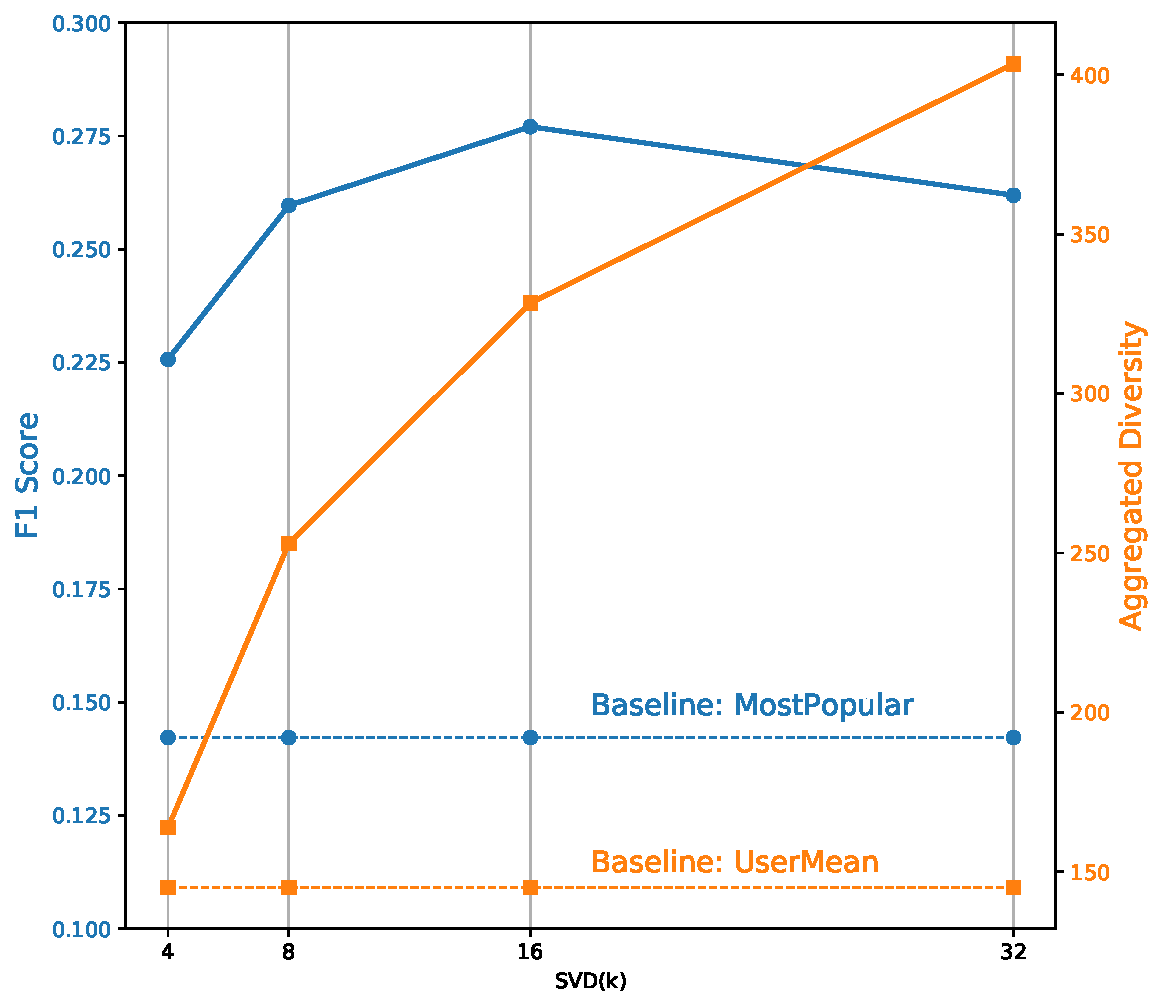
\includegraphics[width=1.0\linewidth]{images/tradeoff.pdf}
    \caption{$F_1$ score (accuracy metric calculated by $2 \frac{\mathrm{recall} \cdot \mathrm{precision}}{\mathrm{recall} + \mathrm{precision}}$) and aggregated diversity (non-accuracy metric) for $\mathrm{SVD}_k$ recommenders, based on the numbers in \tab{results}. The accuracy graph shows that an optimal $k$ is $16$ where $F_1$ score is maximized, whereas diversity monotonically increases as $k$ gets larger. Best baseline metrics are illustrated as dashed lines for reference.}
    \label{fig:tradeoff}
\end{figure}

\begin{table*}[]
    \centering
    \tbl{Results from 5-fold cross-validation of top-10 recommendation conducted on MovieLens 100k user-item-rating pairs. Numbers are rounded to 3 decimal places, and those in the bold font indicate the ``best'' values for each metric. Accuracy metrics for \texttt{MostPopular} are not calculated because the recommender does not explicitly predict ratings.}{
    \begin{tabular}{|cl||r|r|r|r|r|r|r|}
    \hline
    \multicolumn{2}{|c||}{}                                                                                                           & \texttt{ItemMean} & \texttt{UserMean} & \texttt{MostPopular} & \texttt{SVD(4)} & \texttt{SVD(8)} & \texttt{SVD(16)} & \texttt{SVD(32)} \\ \hline \hline
    \multicolumn{1}{|c|}{\multirow{2}{*}{\begin{tabular}[c]{@{}c@{}}Rating\\ (\sect{rating-metrics})\end{tabular}}}         & \texttt{RMSE               } & 0.642    & 0.681    & -           & 0.545  & \textbf{0.524}  & \textbf{0.524}   & 0.550   \\ \cline{2-9} 
    \multicolumn{1}{|c|}{}                                                                                           & \texttt{MAE                } & 0.603    & 0.642    & -           & 0.493  & 0.471  & \textbf{0.470}   & 0.496   \\ \hline \hline
    \multicolumn{1}{|c|}{\multirow{6}{*}{\begin{tabular}[c]{@{}c@{}}Ranking\\ (\sect{ranking-metrics})\end{tabular}}}       & \texttt{Recall             } & 0.108    & 0.002    & 0.114       & 0.182  & 0.212  & \textbf{0.228}   & 0.218   \\ \cline{2-9} 
    \multicolumn{1}{|c|}{}                                                                                           & \texttt{Precision          } & 0.185    & 0.004    & 0.189       & 0.297  & 0.335  & \textbf{0.353}   & 0.328   \\ \cline{2-9} 
    \multicolumn{1}{|c|}{}                                                                                           & \texttt{AUC                } & 0.417    & 0.018    & 0.429       & 0.531  & 0.558  & \textbf{0.579}   & 0.571   \\ \cline{2-9} 
    \multicolumn{1}{|c|}{}                                                                                           & \texttt{ReciprocalRank     } & 0.415    & 0.011    & 0.409       & 0.583  & 0.642  & \textbf{0.670}   & 0.645   \\ \cline{2-9} 
    \multicolumn{1}{|c|}{}                                                                                           & \texttt{MPR                } & 84.671   & 89.784   & 84.021      & 80.192 & 78.431 & \textbf{77.417}  & 78.023  \\ \cline{2-9} 
    \multicolumn{1}{|c|}{}                                                                                           & \texttt{NDCG               } & 0.201    & 0.004    & 0.203       & 0.327  & 0.371  & \textbf{0.392}   & 0.365   \\ \hline \hline
    \multicolumn{1}{|c|}{\multirow{3}{*}{\begin{tabular}[c]{@{}c@{}}Aggregated\\ (\sect{aggregated-metrics})\end{tabular}}} & \texttt{AggregatedDiversity} & 52.2     & 145.0    & 52.4        & 163.8  & 253.0  & 328.4   & \textbf{403.4}   \\ \cline{2-9} 
    \multicolumn{1}{|c|}{}                                                                                           & \texttt{ShannonEntropy     } & 3.149    & 4.170    & 3.160       & 4.486  & 4.847  & 5.138   & \textbf{5.386}   \\ \cline{2-9} 
    \multicolumn{1}{|c|}{}                                                                                           & \texttt{GiniIndex          } & 0.662    & 0.669    & 0.658       & 0.597  & 0.629  & 0.616   & \textbf{0.599}   \\ \hline \hline
    \multicolumn{1}{|c|}{\multirow{2}{*}{\begin{tabular}[c]{@{}c@{}}Intra-list\\ (\sect{intra-list-metrics})\end{tabular}}} & \texttt{Coverage           } & 0.006    & 0.006    & 0.006       & 0.006  & 0.006  & 0.006   & 0.006   \\ \cline{2-9} 
    \multicolumn{1}{|c|}{}                                                                                           & \texttt{Novelty            } & 8.998    & \textbf{9.944}    & 8.970       & 8.763  & 8.751  & 8.991   & 9.424   \\ \hline
    \end{tabular}
    }
    \label{tab:results}
\end{table*}

Meanwhile, rule-based \texttt{UserMean} recommender, which simply scores items by a mean rating per user, was the best in terms of novelty, demonstrating the higher ability to surface unseen items at the top. In combination with the trade-off discussion above, the results tell us that focusing only on a single metric can easily confuse developers and mislead the users of recommender systems. Therefore, it is crucial to holistically assess the systems from multiple perspectives, and the design principle of \texttt{Recommendation.jl} follows the point as we explained in \sect{introduction}.

It should be noticed that, as \texttt{kwargs...} in \sect{intra-list-metrics} indicate, evaluation in intra-list metrics is not straightforward due to the need for specifying additional arguments to set up a scenario. For the sake of simplicity, this section assumes \texttt{catalog} for \texttt{Coverage} is a set of all items available in the dataset, and \texttt{observed} for \texttt{Novelty} is a set of items in target user's training samples, allowing the recommenders to recommend the same items in a training set to the same user. Thus, \texttt{Coverage} in \tab{results} is the same across the recommenders because we always recommend 10 items per user from the fixed set of all items. Moreover, we did not evaluate in \texttt{IntraListSimilarity} and \texttt{Serendipity} because there is no obvious way to define item-item similarities, relevance, and unexpectedness; the choices depend largely on the developer's hypotheses and objectives that this paper does not discuss in detail.


\section{Conclusion}
This paper introduced \texttt{Recommendation.jl}, an open-source package for building recommender systems in the Julia programming language. First, by reviewing each of the core features of practical recommender pipelines, data model (\sect{data}), recommender interface and algorithms (\sect{algorithm}), and evaluation methods (\sect{evaluation}), we observed how diverse recommender's interests can be; the applications must be able to address both explicit and implicit representation of user feedback, hybridize rule-based and machine learning-based algorithms, and assess the outcomes from wide-ranging perspectives in terms of not only accuracy but diversity, coverage, novelty, and serendipity. Thus, Julia's extensible and mathematical operation-friendly APIs come in handy for working with the unique characteristics we demonstrated by their formulation and corresponding code snippet throughout the paper.

Moreover, we conducted a benchmark with multiple recommender-metric pairs provided by \texttt{Recommendation.jl} and confirmed there are no one-size-fits-all approaches to making ``good'' recommendations. On the one hand, we can maximize prediction accuracy by training a sophisticated model-based recommender with an optimal set of hyperparameters. However, at the same time, the best prediction accuracy does not always yield the most diverse recommendation, which might eventually hinder recommenders from acknowledging fairness implications. The observations tell us that one of the most important requirements for recommender frameworks is to make a wide variety of options available for developers while leaving enough space for customization, which \texttt{Recommendation.jl} has tried to incorporate by design.

Finally, there are numerous possible directions to improve the package as we learned from the other open-source solutions in \sect{introduction}. For instance, the availability of state-of-the-art recommendation algorithms makes a framework more promising in a competitive environment in the industry, where Python-based machine learning packages play a dominant role. Meanwhile, since computational efficiency is a key criterion that directly leads to a developer's productivity, the use of acceleration techniques such as distributed multiprocessing and GPU programming would be a mandatory step to undergo. Last but not least, easing to run an end-to-end recommendation pipeline iteratively is a foundational challenge so we can bridge a gap between an offline and online setup. In particular, evaluation phases pose a crucial challenge in reproducibility as mentioned in \sect{evaluation}.


% **************GENERATED FILE, DO NOT EDIT**************

\bibliographystyle{juliacon}
\bibliography{ref.bib}


\end{document}
